\Problem{Great Geek Game-show 3000!}{gameshow}
% author: Jon Marius Venstad

\begin{wrapfigure}{r}{7cm}
\vspace{-5mm}
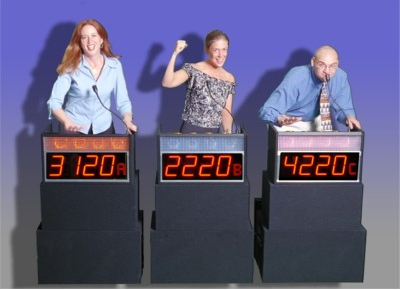
\includegraphics[width=\linewidth,keepaspectratio=true]{gameshow/gameshow}
\vspace{-9mm}
\end{wrapfigure}

\noindent
Yes! You've finally been chosen to participate in the "Great Geek Game-show 3000". This is the moment you've been waiting for, ever since you puzzled out how to maximise your chances of winning. You will finally be rich, and able to buy all the algorithm books you want! Of course you will have to share the winnings with the other contestants, but since your algorithm is vastly superior to the randomness of all the other numb-skulls you are certain you will be able to keep most of the prize money for yourself, in exchange for telling them how you can all maximise your chances of winning.

The rules of the game are the following: There is a stage with $N$ boxes, each containing the name of one of the $N$ contestants, and such that each contestant has their name in exactly one box. The contestants enter the stage one at a time, and each one is allowed to peek inside $K$ of the boxes. If they find their own name inside one of these boxes they can get off the stage, and the game continues with the next contestant. If all contestants find their own name, everyone wins. But if one contestant fails to find theirs, everyone loses. After the game has begun, no communication between the contestants is allowed. 
However you are all allowed to agree upon a strategy before the game begins, and this is where you explain to all the others that the algorithm of everyone choosing $K$ boxes at random is a very bad one, since it gives a chance of winning only equal to ${\frac{K}{N}}^N$. Instead you suggest the following algorithm:

\textit{Assign to each player and each box a unique number in the range $1, \dots, N$. Then each player starts with opening the box with the same number as themselves. The next box the player opens is the box whose number is found inside the first box, then the box whose number is found inside the second box, and so on. The process goes on until the player has opened $K$ boxes, or found their own number.} 

Now to bring home your point of how superior your algorithm is, you will need to calculate the exact odds of winning if all the contestants follow your directions. Unfortunately, this is the only thing you haven't figured out yet \dots 

\Input
One line with the following numbers:\\
$1 \leq N \leq 10000000$ -- the number of contestants.\\
$1 \leq K \leq N$ -- the number of boxes each contestant may check.\\

\Output
The chances you have of winning if everyone follows your algorithm.\\

\Xample{gameshow/gameshow.1}

\Xample{gameshow/gameshow.2}

\Xample{gameshow/gameshow.3}

\Xample{gameshow/gameshow.4}

